\chapter{Entorno experimental}\label{sec:experimentos}

Con el fin de evaluar y medir el rendimiento de \ac{KFC} y \ac{PoFL}, hemos calculado la precisión o \textit{accuracy} del modelo federado resultante en múltiples conjuntos de datos expuestos en la Sección \ref{sec:evaldatasets} donde el objetivo era resolver un problema de clasificación de imágenes. Para esto hemos desplegado modelos basados en \ac{CNN} en un entorno de \ac{FL} explicados en la Sección \ref{sec:modelos}. Finalmente, explicamos los ataques cubiertos en la Sección \ref{sec:ataques}, los escenarios en los que se realizan en la Sección \ref{sec:escenarios} y las métricas usadas para la evaluación en la Sección \ref{sec:metricas}.

\section{Conjuntos de datos para la evaluación}\label{sec:evaldatasets}
Dado que \ac{PoFL}, y por tanto \ac{KFC}, necesitan un conjunto de validación con el fin de medir la precisión de cada modelo de la red, usamos el 20\% del conjunto de test de cada conjunto de datos con este fin dejando el 80\% restante como conjunto de test. Hemos usado tres conjuntos de datos en la evaluación, los cuales describimos a continuación:

\begin{enumerate}
    \item El conjunto de datos EMNIST (\textit{Extended Modified NIST}), presentado en 2017 en \cite{emnist}, es una extensión del famoso conjunto de datos MNIST~\cite{lecun-1998}. La clase \textit{EMNIST Digits} contiene un subconjunto balanceado del conjunto de dígitos. Esta contiene 28,000 muestras de cada dígito. Por lo tanto, el conjunto total consiste en 280,000 muestras, de las cuales 240,000 son usadas para el entrenamiento del modelo y 40,000 como muestras de test (usamos 8,000 como muestras de validación y las 32,000 restantes para test). Para los experimentos hemos decidido establecer el número de clientes en 200 y el de mineros en 3.
    
    \item El conjunto de datos Fashion MNIST \cite{fashionmnist-2017} fue diseñado para ser un reemplazo más exigente del conjunto original MNIST. Contiene un conjunto de 10 clases distintas extraídas del conjunto de imágenes de Zalando con 7,000 muestras de cada clase. Así, el conjunto de datos consiste de 70,000 muestras, de las cuales 60,000 son usadas para entrenamiento y 10,000 para test (usamos 2,000 para validación y las 8,000 restantes para test). Hemos establecido el número de clientes a 200 y el número de mineros a 3.

    \item El conjunto de datos CIFAR-10 es un subconjunto etiquetado del conjunto \textit{80 million tiny images}~\cite{torralba-2008}. Consta de 60,000 imágenes a color de resolución 32x32 de 10 clases, es decir, con 6,000 imágenes por clase. 50,000 imágenes son usadas para entrenamiento y 10,000 como validación, lo que corresponde a 1,000 muestras por clase (usamos 2,000 para validación y las 8,000 restantes para test). Establecemos el número de clientes a 100 (con el fin de tener más datos por cliente pues el modelo a entrenar es mucho más complejo) y el de mineros a 2.
\end{enumerate}


\begin{table}
    \centering
    \begin{tabular}{lrrr}
    \toprule
         &  \textbf{EMNIST}&  \textbf{Fashion MNIST}& \textbf{CIFAR-10}\\
         \toprule
         \textbf{Train}&  240,000&  60,000& 50,000\\
         \midrule
         \textbf{Test}&  32,000&  8,000& 8,000\\
         \midrule
         \textbf{Validation}&  8,000&  2,000& 2,000\\
         \bottomrule
    \end{tabular}
    \caption{Cantidad de muestras en cada conjunto distribuidas según su uso.}
    \label{tab:trainvaltest}
\end{table}

\section{Modelos de clasificación de imágenes}\label{sec:modelos}

Dado que todos los problemas que abordamos son problemas de clasificación, y que el objetivo principal de la propuesta no es maximizar el rendimiento si no probar mecanismos de defensa, usamos modelos de clasificación que obtengan buen rendimiento en estos problemas sin ataques. Para ello hemos considerado dos modelos:

\begin{itemize}
    \item En los conjuntos EMNIST y Fashion MNIST hemos usado una red \ac{CNN} estándar compuesta de dos capas convolucionales seguida cada una por una capas de \textit{max-pooling}, y un clasificador compuesto de dos capas densas con funciones de activación ReLU.
    \item En el conjunto más exigente CIFAR-10, hemos decidido usar una red de la familia ya expuesta previamente EfficientNet, concretamente una \texttt{EfficientNet-B0}. Hemos realizado un \textit{fine-tuning} usando unos pesos preentrenados de la red en el conjunto \textit{ImageNet}.
\end{itemize}

\section{Ataques adversarios}\label{sec:ataques}

A continuación se detallan los ataques implementados, basados en los ya introducidos en la Sección \ref{sec:adversarialattacks}. Con el fin de que las actualizaciones de los clientes adversarios no sean mitigadas al ser agregadas debido a la cantidad de clientes benignos, usamos técnicas de \textit{model replacement} para aumentar la eficacia del ataque.

\subsection{Ataques bizantinos}
Implementamos un ataque bizantino basado en \textit{random label flipping}~\cite{survey-nuria-2023} consistente en cambiar de forma aleatoria las etiquetas de todas las muestras del cliente adversario a una etiqueta distinta de la original. El único objetivo de este ataque es el de perjudicar el rendimiento del modelo federado confundiendo al modelo con las muestras mal etiquetadas.

\begin{figure}[h!]
    \centering
    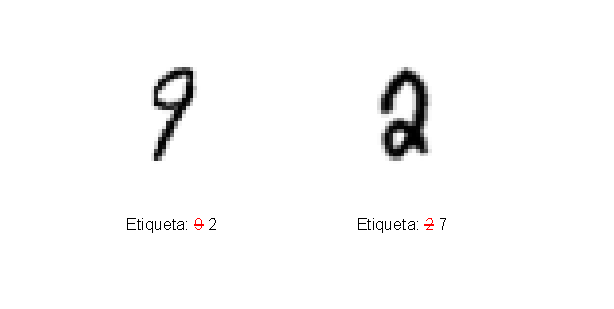
\includegraphics[width=0.8\textwidth]{figuras/labelflipping.pdf}
    \caption{Ejemplo de ataque \textit{random label flipping} en el conjunto de datos EMNIST. Las etiquetas de las muestras son cambiadas por una nueva etiqueta aleatoria manteniendo la muestra original. Fuente: Elaboración propia.}
    \label{fig:enter-label}
\end{figure}

\subsection{Ataques \textit{backdoor} basado en patrones}
También realizamos un ataque de \textit{backdoor} basado en patrones, en el que todos los clientes conocen el patrón completo y lo usan en su proceso de entrenamiento. Establecemos una etiqueta objetivo y un patrón. El número de tareas de \textit{backdoor} es el número de clientes adversarios. Con el fin de demostrar que el comportamiento observado no depende del patrón usado, usamos dos patrones: (1) un píxel blanco en la esquina inferior izquierda para EMNIST y Fashion MNIST o un cuadrado blanco de 5x5 en CIFAR-10, y (2) una cruz blanca de longitud 3 para EMNIST y Fashion MNIST y de longitud 5 para CIFAR-10. La diferencia de tamaño en los patrones se debe al uso del modelo de \textit{EfficientNet} pues este usa un recorte central en la imagen. Se pueden ver los patrones en la Figura \ref{fig:patterns}.

\begin{figure}[h!]
\centering
\begin{subfigure}{.16\linewidth}
  \centering
  
\includegraphics[width=0.8\linewidth]{figuras/backdoor/emnist.png}
  \caption{Imagen.}
  %\label{fig:sfig1}
\end{subfigure}
\begin{subfigure}{.16\linewidth}
  \centering
  
\includegraphics[width=0.8\linewidth]{figuras/backdoor/emnist_cross.png}
  \caption{Cruz.}
  %\label{fig:sfig2}
\end{subfigure}
\begin{subfigure}{.16\linewidth}
  \centering
  
\includegraphics[width=0.8\linewidth]{figuras/backdoor/emnist_square.png}
  \caption{Cuadrado.}
  %\label{fig:sfig3}
\end{subfigure}
\vskip\baselineskip
\begin{subfigure}{.16\linewidth}
  \centering
  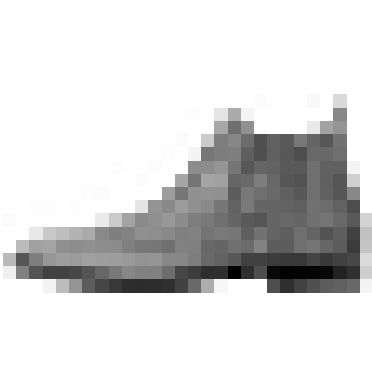
\includegraphics[width=0.8\linewidth]{figuras/backdoor/fashion.png}
  \caption{Imagen.}
  %\label{fig:sfig4}
\end{subfigure}
\begin{subfigure}{.16\linewidth}
  \centering
  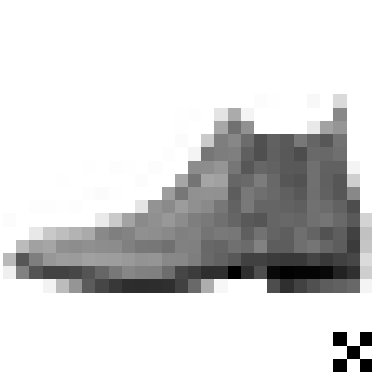
\includegraphics[width=0.8\linewidth]{figuras/backdoor/fashion_cross.png}
  \caption{Cruz.}
  %\label{fig:sfig5}
\end{subfigure}
\begin{subfigure}{.16\linewidth}
  \centering
  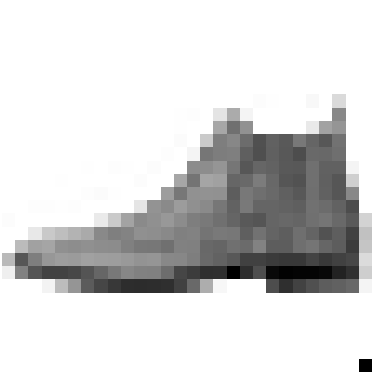
\includegraphics[width=0.8\linewidth]{figuras/backdoor/fashion_square.png}
  \caption{Cuadrado.}
  %\label{fig:sfig6}
\end{subfigure}
\vskip\baselineskip
\begin{subfigure}{.16\linewidth}
  \centering
  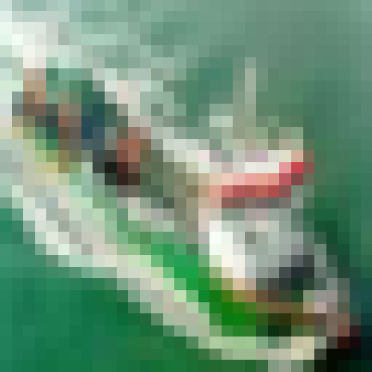
\includegraphics[width=0.8\linewidth]{figuras/backdoor/cifar.png}
  \caption{Imagen.}
  %\label{fig:sfig4}
\end{subfigure}
\begin{subfigure}{.16\linewidth}
  \centering
  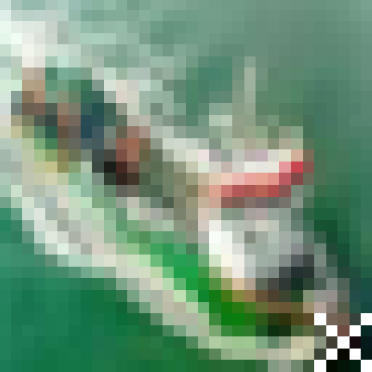
\includegraphics[width=0.8\linewidth]{figuras/backdoor/cifar_cross.png}
  \caption{Cruz.}
  %\label{fig:sfig5}
\end{subfigure}
\begin{subfigure}{.16\linewidth}
  \centering
  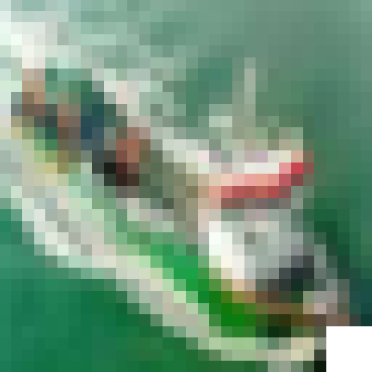
\includegraphics[width=0.8\linewidth]{figuras/backdoor/cifar_square.png}
  \caption{Cuadrado.}
  %\label{fig:sfig6}
\end{subfigure}
\vskip\baselineskip
\caption{Ejemplos de muestras originales (a, d y g) y envenenadas con patrón de cruz (b, e y h), y de cuadrado (c, f and i) en los conjuntos de datos
EMNIST, Fashion-MNIST y CIFAR, respectivamente.}
\label{fig:patterns}
\end{figure}

\section{Escenarios de los ataques}\label{sec:escenarios}
Con el objetivo de poner a prueba nuestras propuestas en distintos entornos consideramos dos escenarios distintos:
\begin{enumerate}
    \item \textbf{Escenario A:} Solo hay un único cliente adversario participando en una ronda de aprendizaje $t$.
    \item \textbf{Escenario B:} La cantidad de clientes adversarios en una ronda de aprendizaje se establece a la cantidad de mineros en la red. En el caso de que la arquitectura a comprobar haga uso de \textit{pooled-mining}, esto es, a cada minero se le asigna un subconjunto de los clientes y no hace uso de ningún tipo de recurso del subconjunto de otro minero, nos aseguramos que cada subconjunto contenga un cliente adversario.
\end{enumerate}

\section{Métricas usadas para la evaluación}\label{sec:metricas}
Consideraremos las métricas según el escenario que estemos cubriendo:

\subsection{Métricas en el caso sin atacantes}
En esta situación nos encontramos ante un caso genérico de clasificación de imágenes. Por lo tanto, usaremos la precisión o \textit{accuracy} en el conjunto de test de nuestro conjunto de datos para medir el rendimiento del modelo.

\subsection{Métricas para ataques bizantinos}
Cuando medimos una defensa contra un ataque bizantino, el objetivo es obtener el mejor rendimiento del modelo en la tarea planteada. Es por ello que comprobamos la precisión o \textit{accuracy} del modelo en el subconjunto de test del conjunto de datos que estamos considerando. Claramente, cuanto mayor sea este valor, mejor será la defensa contra este tipo de ataques.

\subsection{Métricas para ataques de backdoor}
A la hora de defendernos de un ataque de \textit{backdoor}, debemos de considerar dos aspectos distintos. Estos son, el rendimiento del modelo resultante en la tarea original y en la tarea inyectada. La meta es reducir el impacto del ataque lo máximo posible sin comprometer el rendimiento del modelo en la tarea original. Para ello consideramos dos conjuntos de test:
\begin{enumerate}
    \item \textbf{Conjunto de test original}. El conjunto de test original usado para medir el rendimiento en términos de la precisión o \textit{accuracy} en la tarea original.
    \item \textbf{Conjunto de test de \textit{backdoor}}. Este conjunto representa el ataque con el fin de medir el rendimiento de la tarea de \textit{backdoor}. Consiste del conjunto de test original pero envenenado usando el patrón, con el fin de medir la capacidad de generalización del ataque. 
\end{enumerate}

Una defensa será más efectiva cuanto más consiga prevenir el ataque (menor rendimiento en el test de \textit{backdoor}) minimizando la pérdida de rendimiento en la tarea original (mayor rendimiento en el test original).

Dado que los resultados pueden ser altamente heterogéneos en cada ronda de aprendizaje y con el fin de mostrar resultados robustos, mostramos tanto la métrica de la última ronda (\textit{accuracy}) como la media de cada una de estas métricas en las últimas diez rondas de aprendizaje ($accuracy_{10}$). Además, dado que los resultados entre mineros de una misma red pueden diferir en el caso de \ac{PoFL} y \ac{KFC}, mostramos las métricas del mejor minero en términos del rendimiento en la tarea original la cual se supone que puede ser medida en un caso real mediante el conjunto de validación usado en estas arquitecturas.

\section{Arquitecturas de referencia}
Comparamos \ac{KFC} y \ac{PoFL} con las siguientes arquitecturas de \ac{FL}, que representan las referencias clásicas y más estudiadas para \textit{blockchain} aplicado al \ac{FL}:
\begin{enumerate}
    \item \textbf{Cliente-Servidor (C-S)}. No hace ningún uso de \textit{blockchain}. Es uno de los escenarios de \ac{FL} más comunes donde un servidor central actúa como agregador y organiza todo el proceso de aprendizaje.
    \item \textbf{\textit{Proof of Work}}. El mecanismo de consenso donde los mineros compiten en una carrera computacional para resolver un puzzle. El ganador actúa como el agregador para una ronda dada. Consiste en un modelo desacoplado.
    \item \textbf{\textit{Proof of Stake}}. Una arquitectura similar a la anterior pero donde se decide usar \ac{PoS} como mecanismo de consenso como alternativa más eficiente a nivel energético para la red. Consiste en un modelo desacoplado.
\end{enumerate}

En todas las arquitecturas de referencia anteriores y en \ac{PoFL} usamos \ac{FedAvg}~\cite{mcmahan-2023} como el operador de agregación el cual es muchas veces considerado el operador de agregación por defecto para \ac{FL} y el más estudiado en la literatura. Además, dado que \ac{PoW} y \ac{PoS} utilizan la misma arquitectura \textit{blockchain} subyacente hemos decidido combinar los resultados de ambos con el fin de obtener una mayor comprensión y que llamaremos PoW/S.

\section{Detalles de implementación}
Los experimentos han sido realizados usando el framework de simulación de \ac{FL} \texttt{flex}~\cite{flex} y la librería de \ac{AA} \texttt{pytorch}~\cite{pytorch}. Con el fin de simular el comportamiento de una \textit{blockchain} en un escenario federado se ha implementado una librería compañera a \texttt{flex} llamada \texttt{flex-block}~\cite{flex}\footnote{\url{https://github.com/FLEXible-FL/flex-block}}. Además, se adjunta el código realizado\footnote{\url{https://github.com/mariogmarq/kfc-experiments}} para asegurar la reproducibilidad de los experimentos realizados.